\chapter{Déplacements}


Savoir se déplacer est primordial en escrime : cela permet de pouvoir esquiver les attaques, augmenter l'efficacité des frappes ou encore suivre un adversaire qui s'éloigne.
Il est en effet difficile d'imaginer un combat où les deux opposants se font face sans bouger.

Bien que les déplacements ne prennent tout leur sens que lorsqu'ils sont effectués conjointement avec une autre action offensive ou défensive il reste possible d'étudier les notions principales séparément.
C'est ce que nous proposons de faire dans ce chapitre : par la suite nous reviendrons sur les déplacements en association avec les armes, et aussi sur les déplacements spécialisés associés à certains styles.

L'équilibre est une donnée primordiale lors des déplacements : toute période d'équilibre est une opportunité pour l'adversaire et doit donc être réduite au minimum, ou bien être utilisée dans un but précis.
De plus il faut garder à l'idée que l'escrime ne se pratiquait généralement pas sur une surface aussi régulière que dans un gymnase ou avec une tenue légère : les guerriers étaient amenés à combattre à l'extérieur, sur des sols inégaux (boue, dénivelé, trous…), parfois en portant des équipements (armures…).
Il est d'autant plus important de garder à l'esprit la recherche de l'équilibre afin de ne pas s'habituer aux facilités offertes.
En particulier il peut être intéressant de pratiquer en extérieur de temps en temps.


%%%%%%%%%%%%%%%%%%%%%%%%%%%%%%
\section{Déplacements simples}
%%%%%%%%%%%%%%%%%%%%%%%%%%%%%%


% TODO: images

Dans cette section tous les déplacements s'exécutent à partir de la position de garde standard (définition~\ref{struc:def:position-garde}).
De plus la majorité des déplacements terminent en garde (à l'exception de la fente).

Un point important de ne pas \emph{glisser} les pieds lorsque l'on se déplace : cela peut paraître anodin, mais en fait cela diminue la capacité de réagir.
De plus cela serait impossible sur un terrain accidenté, ou du moins dangereux (surtout si l'on porte une armure).

Les deux mouvements de base sont la marche et la retraite et permettent de progresser respectivement vers l'avant et vers l'arrière.
Dans les deux cas le mouvement est de faible amplitude -- moins de la largeur des épaules -- afin de garder l'équilibre et de pouvoir réagir rapidement (par exemple en changeant de direction).
Ainsi on préférera généralement un grand nombre de petits déplacements plutôt que quelques grandes enjambées.
Rappelons que tous ces mouvements se font avec les jambes fléchies.


\begin{definition}[Marche]
\index{déplacement!marche}

La marche correspond à un déplacement vers l'avant de faible amplitude, en avançant d'abord le pied avant suivi du pied arrière.
\end{definition}


\begin{definition}[Retraite]
\index{déplacement!retraite}
\index{déplacement!rompre|see{retraite}}

La marche correspond à un déplacement vers l'arrière de faible amplitude, en reculant d'abord le pied arrière puis le pied avant.

Le verbe correspondant est \emph{rompre}.
\end{definition}


Dans le déplacement latéral on démarre avec le pied qui se trouve du côté désiré afin de ne pas croiser les jambes (et ce quel que soit le pied avant), ce qui induirait un déséquilibre.
À noter que le pied qui se trouve à l'avant reste à l'avant à la fin du mouvement, et de même le pied à l'arrière reste à l'arrière.

% TODO: terme technique ?
\begin{definition}[Marche latérale]
\index{déplacement!marche latérale}

Dans une marche latérale vers la gauche (resp.\ droite), le pied gauche (resp.\ droit) est déplacé en premier vers la gauche (resp.\ droite), puis le pied droit (resp.\ gauche) est déplacé.
\end{definition}


Le changement de garde consiste à échanger les pieds avant et arrière.
Par exemple cela permet de se préparer à attaquer de l'autre côté ou de se défendre plus efficacement.


% marche alternée
\begin{definition}[Changement de garde avant]
\index{déplacement!changement de garde}
\index{garde!changement de --}

Pour un changement de garde avant le pied arrière passe à l'avant, dirigé droit devant, pendant que l'autre pied pivote pour se placer à 45°.
\end{definition}


\begin{definition}[Changement de garde arrière]

Pour un changement de garde arrière le pied avant passe à l'arrière, positionné à 45°, pendant que l'autre pied pivote pour pointer vers l'avant.
\end{definition}


% marche alternée
\begin{definition}[Changement de garde latéral]

Si le pied gauche (resp.\ droit) se trouve à l'avant, alors un changement de garde latéral à droite (resp.\ gauche) consiste à déplacer le pied droit (resp.\ gauche) vers la droite (resp.\ gauche) et en diagonale de sorte à l'amener à la même hauteur que l'autre pied, puis le pied gauche (resp.\ droit) est ramené en arrière.
\end{definition}


\begin{exercice}
\label{ex:general:miroir}

\A et \D se font face et se déplacent en miroir.
\end{exercice}


L'inconvénient des déplacements précédents est de ne pas permettre d'attaquer loin.
Pour ce faire on pourra utiliser une demi-fente afin de gagner en portée, en agrandissant l'écart entre les jambes.
La demi-fente est une action rapide qui s'effectue grâce à la détente de la jambe arrière.
Toutefois cette détente s'effectue au détriment de la mobilité : pour cette raison ne tendra pas totalement la jambe afin de pouvoir garder une certaine liberté de mouvement (la fente, décrite plus loin, va jusqu'au bout du mouvement).
Cela est d'autant plus vrai si l'on se trouve sur un terrain accidenté ou si l'on est alourdi par des protections.
% TODO: vérifier
% Une autre raison est que la fente totale est moins intéressante lorsqu'il s'agit de porter des coups de taille.
En particulier une fois l'attaque effectuée il faudra revenir en garde rapidement.

\begin{definition}[Demi-fente]
\label{dep:def:demi-fente}
\index{déplacement!demi-fente}

La demi-fente consiste à tendre presque entièrement la jambe arrière afin de projeter la jambe avant devant soi.
Le retour en garde se fait en poussant sur la jambe avant et en repliant la jambe arrière.
\end{definition}


\begin{definition}[Remise de fente]
\index{déplacement!remise de fente}

Après une demie-fente, la remise consiste à ramener la jambe arrière juste derrière la jambe avant afin d'exécuter une seconde fente.
\end{definition}


\begin{exercice}
\index{echauffement@échauffement!exercice}

Un meneur indique des déplacements que le reste du groupe doit effectuer : marche, retraite, fente, changement de garde.
Le rythme peut accélérer au fur et à mesure (cela fait un bon exercice d'échauffement).
\end{exercice}


Une manière de prendre l'avantage est de sortir de l'axe : cela consiste à sortir du champ d'attaque naturel de l'adversaire en se déplaçant sur le côté (par exemple avec une marche latérale).
En général ce mouvement s'accompagne d'une attaque afin de profiter d'une ligne ouverte qui sera plus difficile à l'adversaire de protéger (voir le chapitre~\ref{sec:att-def:attaque}).
Dans le cas contraire l'adversaire aura besoin de peu d'efforts pour réaligner son axe.


\begin{definition}[Sortie d'axe]
\label{dep:def:sortie-axe}
\index{déplacement!sortie d'axe}

Sortir de l'axe consiste à s'écarter de la ligne définie par la garde de l'adversaire (voir la figure~\ref{def:fig:sortie-garde}).
\end{definition}


\begin{figure}[ht]
	\centering
	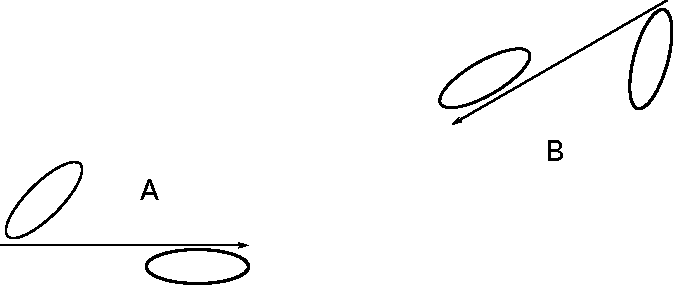
\includegraphics[scale=1]{structure/sortie_axe_pieds.pdf}
	\caption{Illustration d'une sortie d'axe.
	L'axe de B est toujours pointé vers A, mais la réciproque n'est pas vraie.}
	\label{def:fig:sortie-garde}
\end{figure}


%%%%%%%%%%%%%%%%%%%%%%%%%%%%%%%%%
\section{Déplacements techniques}
%%%%%%%%%%%%%%%%%%%%%%%%%%%%%%%%%


Les déplacements décrits dans cette section sont plus avancés et sont utilisés afin de surprendre l'adverse, que ce soit en dissimulant son intention ou en attaquant selon une ligne imprévue.
Toutefois la plupart de ces déplacements présentent une phase de déséquilibre qui peut être exploitée par l'opposant.

Nous allons maintenant décrire plusieurs mouvements, toujours de faible amplitude, qui impliquent de rapprocher les jambes ou de les croiser.
Ainsi que nous l'avons expliquer précédemment cela entraîne un certain déséquilibre, mais qui est compensé par l'ouverture de nouvelles possibilités.

En premier se trouvent les marche et retraite inversées : le pied déplacé en premier est l'inverse de celui déplacé pour une marche/retraite normale.
Dans le cas de la marche inversée l'intérêt est de pouvoir dissimuler plus longtemps le déplacement puisque la jambe arrière est moins visible tout en permettant de bénéficier d'un effet "ressort" : celui-ci peut permettre d'enchaîner efficacement avec une demi-fente au lieu d'une simple marche.
De son côté la retraite inversée peut se transformer en feinte.


\begin{definition}[Marche inversée]
\index{déplacement!marche inversée}

La marche inversée consiste à avancer d'abord le pied arrière juste derrière le pied avant, puis ensuite le pied avant.
\end{definition}


\begin{definition}[Retraite inversée]
\index{déplacement!retraite inversée}

La retraite inversée consiste à reculer d'abord le pied arrière juste derrière le pied avant, puis ensuite le pied avant.
\end{definition}


Dans les mouvements qui suivent les deux pieds se retrouvent croisés.
Ces variations se rencontrent surtout à la rapière.

% quarter du pied ?
\begin{definition}[Marche latérale croisée]
% \index{déplacement!retraite inversée}

Dans une marche latérale croisée vers la gauche (resp.\ droite), le pied droit (resp.\ gauche) est déplacé en premier vers la gauche (resp.\ droite) et dépasse le pied gauche (resp.\ droite), puis le pied droit (resp.\ gauche) est déplacé.
\end{definition}


La demi-fente est une version extrême de la demi-fente (définition~\ref{dep:def:demi-fente}) et utilisée en particulier en escrime moderne.
Son principal défaut est de limiter le mouvement et de nécessiter un certain temps pour revenir en garde du fait que les articulations sont verrouillées.


\begin{definition}[Fente]
\index{déplacement!fente}

La fente consiste à avancer largement le pied en tendant complètement la jambe arrière.
\end{definition}


% TODO: volte, balestra


%%%%%%%%%%%%%%%%
\section{Chutes}
%%%%%%%%%%%%%%%%


Dans cette section nous donnons plusieurs exercices afin de s'entraîner à tomber.
Il s'agit d'une capacité utile dans le cadre de la lutte (au corps-à-corps ou avec des armes) qui implique souvent des projections : les ignorer retire une partie des techniques disponibles et, surtout, de la réalité du combat historique (même si cela n'empêche pas de faire des projections "douces" quand son partenaire n'est pas à l'aise).
En particulier s'entraîner régulièrement permet de perdre la peur de tomber.
Finalement les chutes permettent d'ajouter un élément spectaculaire lors de des spectacles.


% Romain
\noindent
Quelques principes :
\begin{itemize}
	\item chute en avant : mettre les avants bras, ne pas tomber sur les coudes ou les genoux ;
	\item chute en arrière : remonter les épaules pour protéger la tête, se tourner un peu pour atterrir sur l'épaule et pas sur les coudes.
\end{itemize}
Une chute sur une articulation peut faire très mal si l'on porte une armure en plus.


Les trois exercices qui suivent peuvent être être effectués avec une arme (d'abord une canne, puis des armes plus lourdes et encombrantes) une fois que l'on a pris de l'assurance.


\begin{exercice}[Chute]

Se laisser tomber sur un tapis.

\end{exercice}


\begin{exercice}[Chute en hauteur]

Se laisser tomber d'un banc ou d'une table sur un tapis.

% Source : Romain.
\end{exercice}


\begin{exercice}[Roulade par dessus un obstacle]
Mettre un tapis derrière un banc et faire une roulade sur le tapis sans toucher le banc.
\end{exercice}


\begin{exercice}
\A et \D ont leur hanche droite en contact et regardent dans des directions opposées.
\A appuie et fait tomber \D en arrière.

\source{\cite{petit:dijon:close_longword:2015}}
\end{exercice}


\begin{exercice}
\A et \D regardent dans la même direction.
\A a sa hanche gauche contre la hanche droite de \D.
\A appuie sur le torse de \D pour le faire tomber en arrière.

\source{\cite{petit:dijon:close_longword:2015}}
\end{exercice}


\begin{exercice}
Idem que le premier exercice, mais \A mais sa jambe bien plus loin.
En général \D va tomber en avant.

\source{\cite{petit:dijon:close_longword:2015}}
\end{exercice}

